\subsection*{Zadatak Šeširi}
\textsf{Pripremila: Paula Vidas}\\
\textsf{Potrebno znanje: prikazivanje zadatka kao graf}

Raspored šešira možemo promatrati kao binarni niz duljine $N$, gdje $i$-ti bit
predstavlja boju šešira $i$-tog informatičara.
Kako informatičar vidi sve šešire osim svojega, on zna da postoje točno dva moguća
rasporeda šešira, pa ga možemo prikazati kao brid koji spaja te dvije mogućnosti,
a njegovu odluku o boji koju će reći kao usmjerenje tog brida prema onoj mogućnosti
za koju se odlučio.

Drugim riječima imamo graf binarnih nizova duljine $N$, u kojem postoji brid
između svaka dva vrha koji se razlikuju u točno jednom bitu. Ovaj graf zove se još
i \textit{hiperkocka}. Potrebno je naći usmjerenje bridova koje će zadovoljiti
uvjet iz zadatka.

Bridove hiperkocke moguće je obojati u dvije boje tako da za svaki vrh vrijedi da su njegovi
bridovi iste boje ako i samo ako su pripadajući bitovi vrha jednaki. (Boja brida ovisi o tome
da li brid povećava ili smanjuje broj jedinica, ako gledamo od vrha s parno mnogo jedinica
prema vrhu s neparno mnogo jedinica.)

Tada uvjet glasi: za svaki vrh grafa $x$ i svaku od dvije boje bridova $b$, barem pola,
zaokruženo na dolje, bridova iz $x$ boje $b$ mora biti usmjereno prema $x$.

Ako je $N$ paran, svi vrhovi imaju paran stupanj. Ako je $N$ neparan, onda
su svi stupnjevi neparni, te možemo dodati novi vrh u graf i povezati ga sa svim ostalim
vrhovima (bridovima treće boje), i onda će svi stupnjevi postati parni.

\begin{figure}[H]
    \centering
    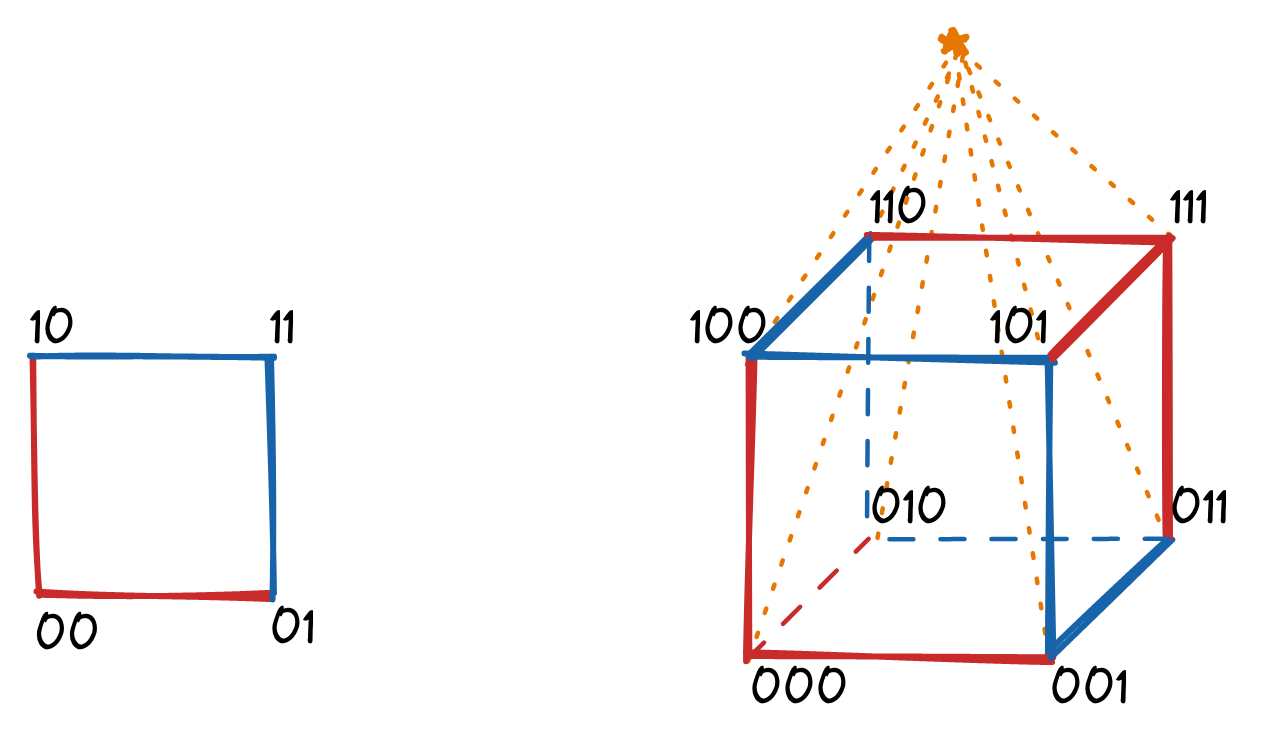
\includegraphics[width=0.6\textwidth]{img/sesiri_editorial.excalidraw.png}
\end{figure}

Sad usmjerenje bridova možemo naći algoritmom koji podsjeća na algoritam za pronalazak
Eulerovog ciklusa. Sve dok nismo usmjerili sve bridove, radimo sljedeće: krenemo iz nekog
vrha koji ima neusmjerenih bridova, te se pomičemo po neusmjerenim bridovima dok možemo i usmjeravamo ih.
Pritom uvijek biramo brid iste boje kao prethodni, ako takav postoji.
Na kraju ćemo se zbog parnosi stupnjeva naći u početnom vrhu i svi njegovi bridovi bit će usmjereni.
